\chapter{Dirac Spinors, Mass, and the Dirac Sea}

These notes follow Leonard Susskind's \emph{Advanced Quantum Mechanics} Lecture 10, curated by LazyingArt LLC. The lecture does not proceed directly to the Dirac sea or to the full three-dimensional Dirac equation. Instead, it backs up and rebuilds the story in the order that makes those later ideas intelligible: first the operator algebra of identical particles, then the one-dimensional Dirac construction, then the three-dimensional massless equation, then the necessity of four components, and only after that the problem of negative energies and antiparticles. Throughout this chapter we use units in which \(\hbar=c=1\).

\section{Exchange Symmetry and Field Algebra}

Susskind begins with the most concrete distinction between bosons and fermions: what happens when two identical particles are interchanged. For bosons the two-particle state is symmetric, while for fermions it is antisymmetric:
\begin{equation}
\lvert x,y\rangle=\lvert y,x\rangle,
\qquad
\lvert x,y\rangle=-\,\lvert y,x\rangle.
\end{equation}
Here \(x\) and \(y\) label the positions of particle \(1\) and particle \(2\); they are not Cartesian coordinates by themselves, but placeholders for points in space.

The state with one particle at \(x\) and one at \(y\) is built from the vacuum by creation operators,
\begin{equation}
\lvert x,y\rangle=\psi^\dagger(x)\psi^\dagger(y)\lvert 0\rangle.
\end{equation}
For bosons this construction must be unchanged when the two operators are interchanged, so the creation operators commute. For fermions the state must change sign, so the creation operators must anti-commute:
\begin{equation}
\psi^\dagger(x)\psi^\dagger(y)\lvert 0\rangle
=
-\,\psi^\dagger(y)\psi^\dagger(x)\lvert 0\rangle,
\end{equation}
and therefore
\begin{equation}
\psi^\dagger(x)\psi^\dagger(y)+\psi^\dagger(y)\psi^\dagger(x)=0,
\qquad
\{\psi^\dagger(x),\psi^\dagger(y)\}=0.
\end{equation}
This is the first important payoff of the exchange rule: the minus sign in the state is enforced by anti-commuting field operators.

\begin{figure}[ht]
\centering

\includegraphics[width=0.78\textwidth]{lecture_10_frame_01.png}
\caption{The board state for the fermionic exchange-sign discussion and the equal-point anti-commutator step. The transcript provides the logical sequence; the figure is retained as local evidence for the order and placement of the exclusion argument.}
\label{fig:aqm10-frame1}
\end{figure}

The lecture then immediately specializes to the case \(y=x\). The transcript is garbled at one intermediate line, but the argument itself is completely clear and is also visible on the board. Setting \(y=x\) gives
\begin{equation}
\{\psi^\dagger(x),\psi^\dagger(x)\}=0,
\end{equation}
so that
\begin{align}
\psi^\dagger(x)\psi^\dagger(x)+\psi^\dagger(x)\psi^\dagger(x)&=0,\\
2(\psi^\dagger(x))^2&=0,\\
(\psi^\dagger(x))^2&=0.
\end{align}
Trying to create two identical fermions in the same state produces the zero vector, not a new state. This is the operator form of the exclusion principle.

\begin{figure}[ht]
\centering
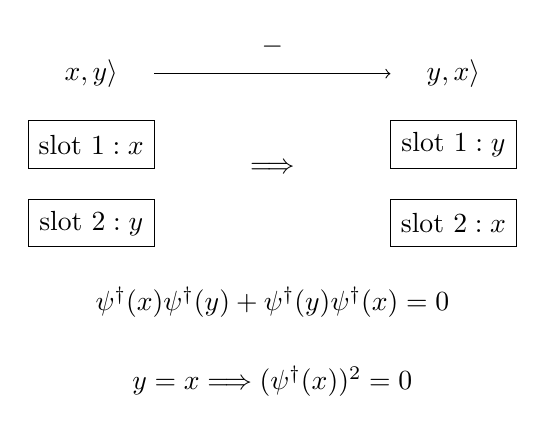
\begin{tikzpicture}[x=1cm,y=1cm]
\node at (0,2.2) {$\lvert x,y\rangle$};
\node at (4.6,2.2) {$\lvert y,x\rangle$};
\draw[->] (0.8,2.2) -- (3.8,2.2);
\node at (2.3,2.55) {$-$};

\draw ( -0.8,1.0) rectangle (0.8,1.6);
\draw ( 3.8,1.0) rectangle (5.4,1.6);
\node at (0,1.3) {slot \(1:x\)};
\node at (4.6,1.3) {slot \(1:y\)};

\draw ( -0.8,0.0) rectangle (0.8,0.6);
\draw ( 3.8,0.0) rectangle (5.4,0.6);
\node at (0,0.3) {slot \(2:y\)};
\node at (4.6,0.3) {slot \(2:x\)};

\node at (2.3,1.0) {$\Longrightarrow$};

\node[align=center] at (2.3,-0.7)
{$\psi^\dagger(x)\psi^\dagger(y)+\psi^\dagger(y)\psi^\dagger(x)=0$};

\node[align=center] at (2.3,-1.7)
{$y=x \Longrightarrow (\psi^\dagger(x))^2=0$};
\end{tikzpicture}
\caption{Transcript-based reconstruction of the logical chain used in the lecture: exchange antisymmetry first, operator anti-commutation second, equal-point exclusion last.}
\label{fig:aqm10-exchange-reconstruction}
\end{figure}

\section{Occupation Numbers and the Algebraic Contrast Between Bosons and Fermions}

Susskind does not leave the discussion at the equal-point anti-commutator. He next asks what the algebra says about creation and annihilation operators themselves.

For a single bosonic mode, the standard support relation is
\begin{equation}
[a,a^\dagger]=1.
\end{equation}
This is enough to make creation and annihilation operators algebraically distinguishable. If the order is reversed,
\begin{equation}
[a^\dagger,a]=-1,
\end{equation}
so even without any physical labels one can tell which symbol is playing which role. This matches the structure of the bosonic occupation ladder:
\begin{equation}
n=0,1,2,\dots.
\end{equation}
A creation operator never runs out of states above it; an annihilation operator eventually hits the bottom and gives zero.

For a single fermionic mode, the corresponding support relations are
\begin{equation}
\{a,a^\dagger\}=1,
\qquad
a^2=0,
\qquad
(a^\dagger)^2=0.
\end{equation}
Now the anti-commutator is unchanged when the order is interchanged. Algebraically, creation and annihilation look much more symmetric. This matches the occupation-number structure of a single fermionic state:
\begin{equation}
n=0 \quad \text{or} \quad n=1.
\end{equation}
The creation operator takes the empty state to the filled state and then kills the state if applied again; the annihilation operator takes the filled state to the empty state and kills the state if applied once more. In this precise sense there is a symmetry between empty and filled.

That symmetry is not merely a side remark. Susskind explicitly flags it as something that will return later. When the lecture reaches negative-energy states, this near-interchangeability of fermionic creation and annihilation operators becomes the algebraic doorway to antiparticles.

\begin{figure}[ht]
\centering
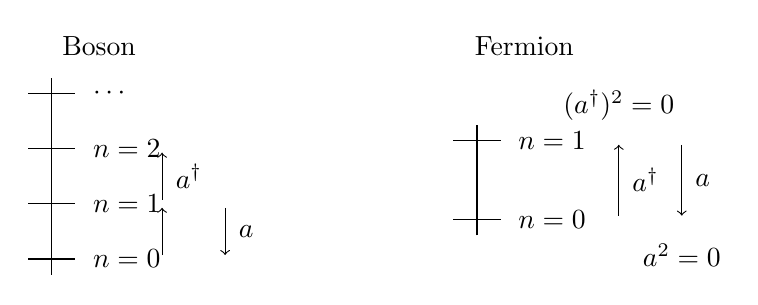
\begin{tikzpicture}[x=1cm,y=1cm]
\node at (0,3.2) {Boson};
\draw (-0.6,0.3) -- (-0.6,2.8);
\foreach \y/\lab in {0.5/{$n=0$},1.2/{$n=1$},1.9/{$n=2$},2.6/{$\cdots$}}
{
  \draw (-0.9,\y) -- (-0.3,\y);
  \node[right] at (-0.2,\y) {\lab};
}
\draw[->] (0.8,0.55) -- (0.8,1.15);
\draw[->] (0.8,1.25) -- (0.8,1.85);
\node[right] at (0.85,1.55) {$a^\dagger$};
\draw[->] (1.6,1.15) -- (1.6,0.55);
\node[right] at (1.65,0.85) {$a$};

\node at (5.4,3.2) {Fermion};
\draw (4.8,0.8) -- (4.8,2.2);
\draw (4.5,1.0) -- (5.1,1.0);
\draw (4.5,2.0) -- (5.1,2.0);
\node[right] at (5.2,1.0) {$n=0$};
\node[right] at (5.2,2.0) {$n=1$};
\draw[->] (6.6,1.05) -- (6.6,1.95);
\node[right] at (6.65,1.5) {$a^\dagger$};
\draw[->] (7.4,1.95) -- (7.4,1.05);
\node[right] at (7.45,1.5) {$a$};
\node at (6.6,2.45) {$(a^\dagger)^2=0$};
\node at (7.4,0.55) {$a^2=0$};
\end{tikzpicture}
\caption{Transcript-based reconstruction of the occupation-number contrast emphasized in the lecture. The bosonic ladder is semi-infinite, while a single fermionic mode has only the states \(n=0\) and \(n=1\).}
\label{fig:aqm10-occupation}
\end{figure}

\section{A One-Dimensional Dirac Review}

Only after this operator review does Susskind return to the Dirac equation. He starts with the simplest one-dimensional massless model,
\begin{equation}
i\,\frac{\partial}{\partial t}\psi_1
=
-\,i\,\frac{\partial}{\partial x}\psi_1,
\end{equation}
which he immediately reads as the Schr\"odinger equation with Hamiltonian
\begin{equation}
H\psi_1=p\,\psi_1.
\end{equation}
This is a one-dimensional relativistic particle with \(E=p\): massless, linear in momentum, and rigidly right-moving. In the language of the earlier reference-book discussion, the wave packet simply propagates to the right at fixed speed.

\begin{figure}[ht]
\centering

\includegraphics[width=0.72\textwidth]{lecture_10_frame_02.png}
\caption{The board state for the one-dimensional Dirac review. The visible equation \(i\partial_t\psi_1=-i\partial_x\psi_1\) and the Hamiltonian form \(H\psi_1=p\psi_1\) are directly supported by the board; the lower \(\psi_2\) line is completed from the transcript.}
\label{fig:aqm10-frame2}
\end{figure}

As it stands, this is not a satisfactory theory of an electron moving on a wire, because it has no mass and only one direction of propagation. So Susskind introduces a second species,
\begin{equation}
H\psi_2=-\,p\,\psi_2.
\end{equation}
A convenient transcript-assisted completion of the board is
\begin{equation}
i\,\frac{\partial}{\partial t}\psi_2
=
+\,i\,\frac{\partial}{\partial x}\psi_2,
\end{equation}
which indeed describes a left-moving wave. The new ingredient is not momentum itself, but a two-valued internal label telling us whether the particle belongs to the right-moving or left-moving species.

He then packages the two into a column vector,
\begin{equation}
\Psi=
\begin{pmatrix}
\psi_1\\
\psi_2
\end{pmatrix},
\end{equation}
and introduces a matrix \(\alpha\) whose eigenvalues distinguish the two sectors:
\begin{equation}
\alpha\psi_1=+\psi_1,
\qquad
\alpha\psi_2=-\psi_2.
\end{equation}
The two equations can now be written at once as
\begin{equation}
H\Psi=\alpha\,p\,\Psi.
\end{equation}
This doubles the number of components, but it still does not produce a mass. For that Susskind adds a second matrix \(\beta\) and writes
\begin{equation}
H=\alpha p+\beta m.
\end{equation}
The important point is algebraic, not representational:
\begin{equation}
\alpha^2=1,
\qquad
\beta^2=1,
\qquad
\alpha\beta+\beta\alpha=0.
\end{equation}
He explicitly warns not to confuse this matrix anti-commutation with the anti-commutation of the fermion field operators. They are different pieces of mathematics serving different purposes.

The reason for the choice becomes clear when \(H\) is squared:
\begin{align}
H^2
&=
(\alpha p+\beta m)^2 \\
&=
\alpha^2 p^2+\beta^2 m^2+(\alpha\beta+\beta\alpha)pm \\
&=
p^2+m^2.
\end{align}
Thus the linear Hamiltonian produces the relativistic dispersion relation
\begin{equation}
E^2=p^2+m^2.
\end{equation}
This is the lecture's first worked example of a general Dirac strategy: enlarge the space of states until a linear Hamiltonian can square to the desired relativistic invariant.

The corresponding physical picture is only partial, but it is pedagogically important in the lecture: the off-diagonal mass term couples right-moving and left-moving sectors. In that sense mass is what makes it meaningful to think of a particle as able to turn around, and hence as able, in a rough picture, to sit at rest.

\begin{figure}[ht]
\centering
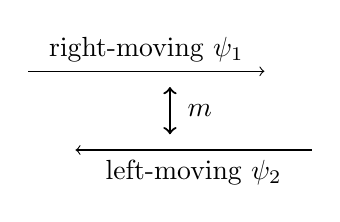
\begin{tikzpicture}[x=1cm,y=1cm]
\draw[->] (0,1.5) -- (3,1.5);
\node[above] at (1.5,1.5) {right-moving \(\psi_1\)};
\draw[->] (3.6,0.5) -- (0.6,0.5);
\node[below] at (2.1,0.5) {left-moving \(\psi_2\)};
\draw[<->,thick] (1.8,1.3) -- (1.8,0.7);
\node[right] at (1.9,1.0) {\(m\)};
\end{tikzpicture}
\caption{Transcript-based reconstruction of the one-dimensional massive picture. The lecture's point is not that the mass term literally describes a classical bounce, but that it couples the left-moving and right-moving sectors.}
\label{fig:aqm10-left-right-mixing}
\end{figure}

\section{Three Dimensions and the Return of Spin}

The lecture now asks how to repeat the same idea in real three-dimensional space. Here the key motivation is rotational invariance. Momentum is a vector, so whatever multiplies it in a linear Hamiltonian must also behave like a vector. One therefore tries
\begin{equation}
H=\boldsymbol{\alpha}\cdot\mathbf p
=
\alpha_x p_x+\alpha_y p_y+\alpha_z p_z.
\end{equation}
To describe a massless relativistic particle we want
\begin{equation}
H^2=\mathbf p^2=p_x^2+p_y^2+p_z^2.
\end{equation}
Squaring \(H\) shows immediately what the matrices must do:
\begin{equation}
\alpha_x^2=\alpha_y^2=\alpha_z^2=1,
\qquad
\alpha_i\alpha_j+\alpha_j\alpha_i=0
\quad
(i\neq j).
\end{equation}
Susskind's question is therefore: can one find three matrices that square to \(1\) and mutually anti-commute? The answer is yes; the Pauli matrices do exactly this. The visible board equations support
\begin{equation}
\alpha_x=\sigma_x=
\begin{pmatrix}
0&1\\
1&0
\end{pmatrix},
\qquad
\alpha_y=\sigma_y=
\begin{pmatrix}
0&-i\\
i&0
\end{pmatrix},
\qquad
\alpha_z=\sigma_z=
\begin{pmatrix}
1&0\\
0&-1
\end{pmatrix},
\end{equation}
where the \(\sigma_z\) entry is the standard completion consistent with the transcript.

\begin{figure}[ht]
\centering

\includegraphics[width=0.70\textwidth]{lecture_10_frame_03.png}
\caption{Board evidence for the transition to the three-dimensional massless Dirac equation. The visible identifications \(\alpha_x=\sigma_x\) and \(\alpha_y=\sigma_y\) mark the moment where the lecture leaves the one-dimensional review and enters the three-dimensional construction.}
\label{fig:aqm10-frame3}
\end{figure}

Thus the three-dimensional massless Hamiltonian becomes
\begin{equation}
H=\boldsymbol{\sigma}\cdot\mathbf p.
\end{equation}
This is the lecture's first explicit appearance of spin. The point is not that spin was inserted by hand because one already knew electrons had magnetic moments. Susskind stresses the opposite: once Dirac insists on a Hamiltonian linear in momentum whose square is \(\mathbf p^2\), the Pauli matrices appear, and with them the spin structure.

The physical interpretation is immediate. In the lecture's normalization, the spin component along the momentum direction has eigenvalues \(\pm1\). Therefore
\begin{equation}
E=\boldsymbol{\sigma}\cdot\mathbf p
\end{equation}
is positive when spin is aligned with momentum and negative when it is anti-aligned. A positive-energy massless particle of this type has its spin locked to its momentum direction. This is the lecture's route to helicity.

\begin{figure}[ht]
\centering
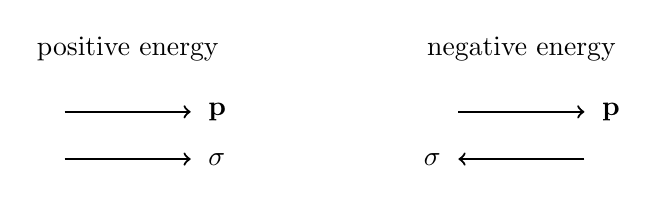
\begin{tikzpicture}[x=1cm,y=1cm]
\node at (0,2.2) {positive energy};
\draw[->,thick] (-0.8,1.4) -- (0.8,1.4);
\draw[->,thick] (-0.8,0.8) -- (0.8,0.8);
\node[right] at (0.9,1.4) {\(\mathbf p\)};
\node[right] at (0.9,0.8) {\(\boldsymbol{\sigma}\)};
\node at (5.0,2.2) {negative energy};
\draw[->,thick] (4.2,1.4) -- (5.8,1.4);
\draw[->,thick] (5.8,0.8) -- (4.2,0.8);
\node[right] at (5.9,1.4) {\(\mathbf p\)};
\node[left] at (4.1,0.8) {\(\boldsymbol{\sigma}\)};
\end{tikzpicture}
\caption{Transcript-based helicity sketch corresponding to \(H=\boldsymbol{\sigma}\cdot\mathbf p\). In the positive-energy sector the spin is aligned with the momentum; in the negative-energy sector it is anti-aligned.}
\label{fig:aqm10-helicity}
\end{figure}

\section{Why Two Components Fail, and Why Four Work}

At this point the lecture pauses to ask whether one can simply add a mass term to the two-component three-dimensional theory:
\begin{equation}
H=\boldsymbol{\sigma}\cdot\mathbf p+\beta m.
\end{equation}
If \(\beta^2=1\), the square of this Hamiltonian contains the desired \(m^2\) term, but it also contains cross terms:
\begin{equation}
p_x m(\sigma_x\beta+\beta\sigma_x),
\qquad
p_y m(\sigma_y\beta+\beta\sigma_y),
\qquad
p_z m(\sigma_z\beta+\beta\sigma_z).
\end{equation}
To remove them one would need
\begin{equation}
\sigma_x\beta+\beta\sigma_x=0,
\qquad
\sigma_y\beta+\beta\sigma_y=0,
\qquad
\sigma_z\beta+\beta\sigma_z=0.
\end{equation}
But no \(2\times2\) matrix exists that anti-commutes with all three Pauli matrices. The obstruction is algebraic and is the decisive failure that drives the lecture to four-component spinors.

Susskind's next move is to enlarge the internal space once again. One convenient representation, matching his block-matrix description, is
\begin{equation}
\alpha_i=
\begin{pmatrix}
\sigma_i&0\\
0&-\sigma_i
\end{pmatrix},
\qquad
\beta=
\begin{pmatrix}
0&I\\
I&0
\end{pmatrix}.
\end{equation}
These matrices satisfy
\begin{equation}
\alpha_i^2=1,
\qquad
\beta^2=1,
\qquad
\alpha_i\alpha_j+\alpha_j\alpha_i=0\ \ (i\neq j),
\qquad
\alpha_i\beta+\beta\alpha_i=0.
\end{equation}
The Hamiltonian
\begin{equation}
H=\boldsymbol{\alpha}\cdot\mathbf p+\beta m
\end{equation}
then obeys
\begin{equation}
H^2=\mathbf p^2+m^2.
\end{equation}

\begin{figure}[ht]
\centering
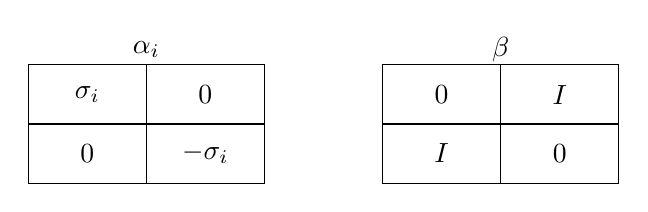
\begin{tikzpicture}[x=1cm,y=1cm]
\node at (1.5,3.1) {$\alpha_i$};
\draw (0,1.4) rectangle (3,2.9);
\draw (1.5,1.4) -- (1.5,2.9);
\draw (0,2.15) -- (3,2.15);
\node at (0.75,2.52) {$\sigma_i$};
\node at (2.25,2.52) {$0$};
\node at (0.75,1.78) {$0$};
\node at (2.25,1.78) {$-\sigma_i$};

\node at (6.0,3.1) {$\beta$};
\draw (4.5,1.4) rectangle (7.5,2.9);
\draw (6.0,1.4) -- (6.0,2.9);
\draw (4.5,2.15) -- (7.5,2.15);
\node at (5.25,2.52) {$0$};
\node at (6.75,2.52) {$I$};
\node at (5.25,1.78) {$I$};
\node at (6.75,1.78) {$0$};
\end{tikzpicture}
\caption{Transcript-based block-matrix panel for a convenient \(4\times4\) representation. The lecture emphasizes that the representation is not unique; the algebra is the essential point.}
\label{fig:aqm10-dirac-blocks}
\end{figure}

This enlargement also clarifies the lecture's chirality story. A two-component massless theory carries only one handedness. The four-component theory contains both handednesses, and the off-diagonal mass term mixes them. That is the precise sense in which the lecture says that mass couples left-handed and right-handed sectors.

\section{Velocity, Zitterbewegung, and Genuine Spin}

Once the \(4\times4\) algebra is in place, Susskind changes emphasis. The problem is no longer how to build the Hamiltonian, but how to interpret the matrices that now appear in it.

He first asks what physical observable the \(\alpha_i\) represent. The answer is obtained from the Heisenberg equation. Susskind explicitly says that he is not going to pause over the overall sign convention, so we choose one consistent convention and write
\begin{equation}
\dot L=i[H,L].
\end{equation}
Applying this to the position operator \(x\) gives
\begin{align}
\dot x
&=
i[H,x] \\
&=
i[\boldsymbol{\alpha}\cdot\mathbf p+\beta m,x] \\
&=
i[\alpha_x p_x,x] \\
&=
i\,\alpha_x[p_x,x] \\
&=
\alpha_x,
\end{align}
where \(\beta\) and the \(\alpha_i\) commute with \(x\) because they act in spinor space rather than in position space, and \([p_x,x]=-i\) in the present units.

So \(\alpha_x\) is the velocity operator. This is the lecture's striking conclusion: the velocity is not simply proportional to the momentum. Since the eigenvalues of \(\alpha_x\) are \(\pm1\), a direct measurement of one velocity component can only yield \(\pm1\).

But \(\alpha_x\) is not conserved. Indeed,
\begin{equation}
\dot\alpha_x=i[H,\alpha_x],
\end{equation}
and the Hamiltonian contains \(\alpha_y\) and \(\alpha_z\), which do not commute with \(\alpha_x\). Therefore
\begin{equation}
[H,\alpha_x]\neq0.
\end{equation}
The resulting rapid, oscillatory motion is the famous \emph{zitterbewegung}. In Susskind's presentation this is not a correction term; it is a direct consequence of the Dirac algebra.

He then insists on a second distinction: \(\alpha_i\) are not the genuine spin. They form an ordinary vector under spatial reflections, whereas spin is an axial vector. In the same block notation, the genuine spin operator is more naturally represented by
\begin{equation}
\Sigma_i=
\begin{pmatrix}
\sigma_i&0\\
0&\sigma_i
\end{pmatrix}.
\end{equation}
Thus a Dirac particle carries several layers of internal structure: chirality or handedness, represented by the way the upper and lower sectors are related, and genuine spin, represented by \(\Sigma_i\). The lecture's interpretive point is that these should not be conflated.

For slowly moving particles the time-averaged motion reproduces the expected classical relation between momentum and velocity, but the exact operator statement remains the strange one: the instantaneous velocity is \(\alpha\), not \(p/m\).

\section{Negative Energies, the Dirac Sea, and the Field Operator}

The lecture's final major pivot is historical and conceptual. To expose the negative-energy problem, Susskind does not need the full three-dimensional theory. He deliberately retreats to the simplest right-moving model,
\begin{equation}
H=P.
\end{equation}
This already has both positive and negative energies, because the momentum eigenvalue \(p\) can be positive or negative. That is dangerous: if negative-energy one-particle states are available, then the supposed vacuum is not the state of lowest energy, since one could always lower the energy by creating more particles in negative-energy states.

The crucial difference between bosons and fermions now returns. If the particles were bosons, there would be no bottom: one could keep piling more particles into the same negative-energy state. But for fermions, exclusion allows only one particle in each state. Dirac's proposal is therefore to define the vacuum as the state in which all negative-energy fermion states are already filled.

\begin{figure}[ht]
\centering
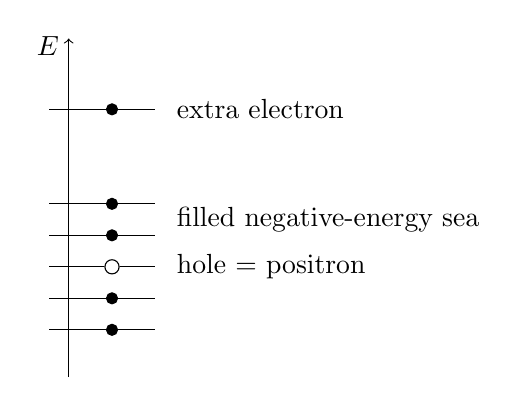
\begin{tikzpicture}[x=1cm,y=1cm]
\draw[->] (0,0) -- (0,4.3);
\node[left] at (0,4.2) {$E$};

\foreach \y in {0.6,1.0,1.4,1.8,2.2}
{
  \draw (-0.25,\y) -- (1.1,\y);
  \filldraw (0.55,\y) circle (0.07);
}

\draw (-0.25,3.4) -- (1.1,3.4);
\filldraw (0.55,3.4) circle (0.07);

\draw (-0.25,1.4) -- (1.1,1.4);
\filldraw[white] (0.55,1.4) circle (0.09);
\draw (0.55,1.4) circle (0.09);
\node[right] at (1.25,1.4) {hole \(=\) positron};

\node[right] at (1.25,3.4) {extra electron};
\node[right] at (1.25,2.0) {filled negative-energy sea};
\end{tikzpicture}
\caption{Transcript-based reconstruction of the Dirac-sea picture used in the lecture. Filling all negative-energy fermion states stabilizes the vacuum; removing one filled negative-energy electron leaves a hole, interpreted as a positron.}
\label{fig:aqm10-dirac-sea}
\end{figure}

Once the sea is filled, one cannot lower the energy further by adding more negative-energy electrons. The vacuum is stable. Excitations above this vacuum can then be described in two ways. One may add a positive-energy electron, or one may remove a negative-energy electron. The second operation creates a hole. Since the removed particle carried negative charge, the hole carries positive charge. Since removing a negative-energy particle raises the energy, the hole has positive energy. That hole is the positron.

The lecture then shifts from the historical sea picture to operator language. The fermion field is written, schematically, as an integral over all momenta. Because the late discussion treats Fourier-sign conventions casually, it is best to preserve only the structural decomposition:
\begin{equation}
\psi(x)\sim
\int_0^\infty dp\, a(p)e^{-ipx}
+
\int_0^\infty dp\, b^\dagger(p)e^{+ipx}.
\end{equation}
The first term annihilates positive-energy electrons; the second creates positrons. Algebraically, this is precisely where the earlier symmetry of fermionic creation and annihilation operators becomes useful: the annihilation of a filled negative-energy electron state can be relabeled as the creation of a positron.

The same field operator then packages several processes at once. Susskind's example is the interaction term
\begin{equation}
H_{\mathrm{int}}\sim \psi^\dagger(x)\psi(x)A(x),
\end{equation}
where \(A\) is the photon field or photon operator. Once the electron and positron pieces are substituted, the single operator product contains the schematic structures
\begin{equation}
a^\dagger a\,A,
\qquad
ba\,A,
\qquad
a^\dagger b^\dagger A,
\end{equation}
corresponding respectively to electron scattering, electron--positron annihilation, and pair creation. In the lecture this is the immediate precursor to the Feynman-diagram viewpoint: one compact operator structure encodes many physical channels.

\begin{figure}[ht]
\centering
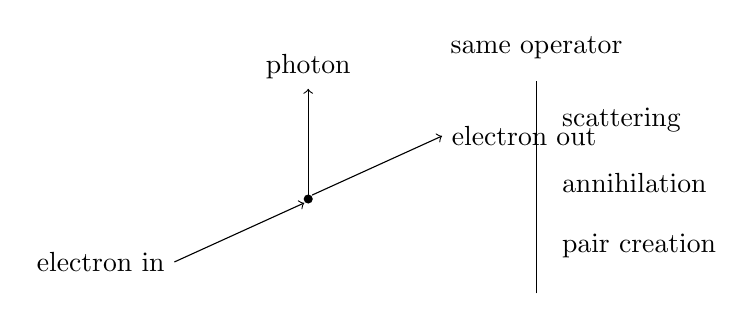
\begin{tikzpicture}[x=1cm,y=1cm]
\filldraw (2.5,1.8) circle (0.05);
\draw[->] (0.8,1.0) -- (2.45,1.75);
\draw[->] (2.55,1.85) -- (4.2,2.6);
\draw[->] (2.5,1.85) -- (2.5,3.2);
\node[left] at (0.8,1.0) {electron in};
\node[right] at (4.2,2.6) {electron out};
\node[above] at (2.5,3.2) {photon};

\draw (5.4,0.6) -- (5.4,3.3);
\node[above] at (5.4,3.45) {same operator};
\node[right] at (5.6,2.8) {scattering};
\node[right] at (5.6,2.0) {annihilation};
\node[right] at (5.6,1.2) {pair creation};
\end{tikzpicture}
\caption{Transcript-based interaction panel for \( \psi^\dagger\psi A \). The lecture's point is not the detailed Feynman rule but the multiplicity of channels contained in a single operator structure once the fermion field is split into electron and positron pieces.}
\label{fig:aqm10-interaction}
\end{figure}

Susskind closes by contrasting two viewpoints. Historically, the filled sea is a vivid and effective picture. In modern operator language one simply flips negative-energy annihilation operators into positive-energy antiparticle creation operators, and the formalism becomes symmetric between electrons and positrons. He then notes that the same pattern appears again in solid-state physics: a filled Fermi sea, an excited electron above it, and a hole behaving as a positively charged excitation.

\section{Summary}

This lecture is built as a sequence of motivated enlargements. Exchange antisymmetry leads to field anti-commutation, equal-point anti-commutation yields exclusion, and the finite occupation structure of fermions prepares the later reinterpretation of holes as particles. The one-dimensional Dirac review shows why a linear Hamiltonian needs extra components to acquire a mass, while the three-dimensional construction forces the Pauli matrices and therefore spin. The failure of a \(2\times2\) mass term pushes the theory to four-component spinors, where mass appears as a coupling between opposite chiralities. Finally, the negative-energy problem is resolved first by Dirac's sea picture and then by the operator reinterpretation in which the fermion field naturally contains both electron annihilation and positron creation.